\FloatBarrier
\subsection{RLS identification with sudden parameter change}

This section utilizes the Simulink model shown \autoref{fig:RLSISPCSimulinModel}. The system has a white noise input with a variance of $2$ and there is a white noise on the output of the system.
The system's $b_2$ parameter transitions from $1$ to $0.5$ at sample number $50$ And parameter $a_3$ change form $\frac{1}{6}$ to $\frac{1}{12}$ at sample number $200$.

\begin{figure}
	\centering
	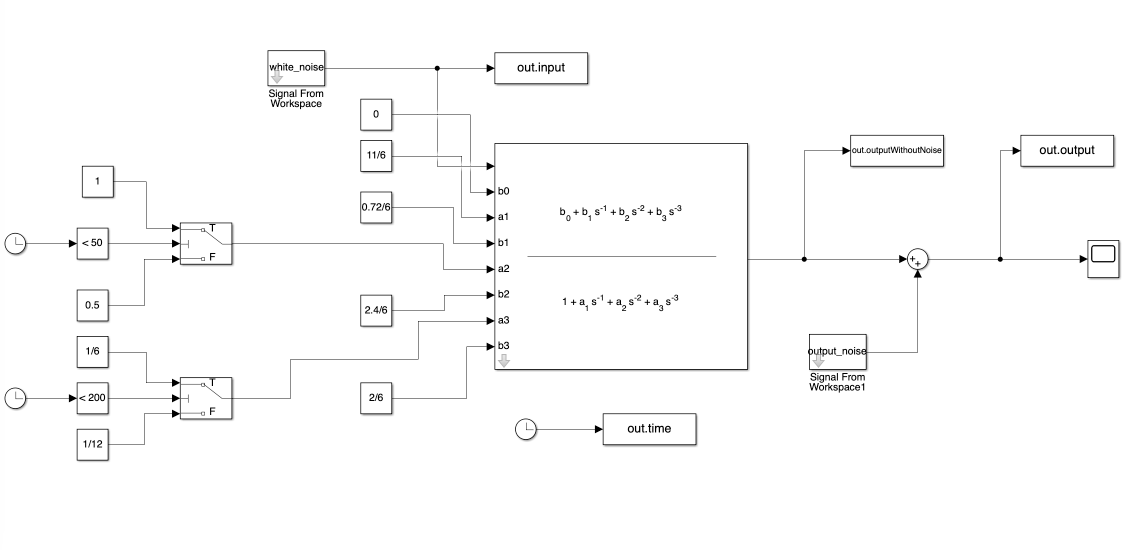
\includegraphics[totalheight=8cm]{images/RLSISPCSimulinkModel.png}
	\caption{RLS system output with sudden change}
	\label{fig:RLSISPCSimulinModel}
\end{figure}

\autoref{fig:RLSISPCOutput} displays the system's output and associated error calculations. \autoref{fig:RLSISPCParams} illustrates the parameter evaluation throughout the program's execution. The final identified transfer function is shown in \autoref{eq:RLSISPCTransferFunction}. To improve parameter estimation, we incorporated a forgetting factor.

\begin{figure}
\centering
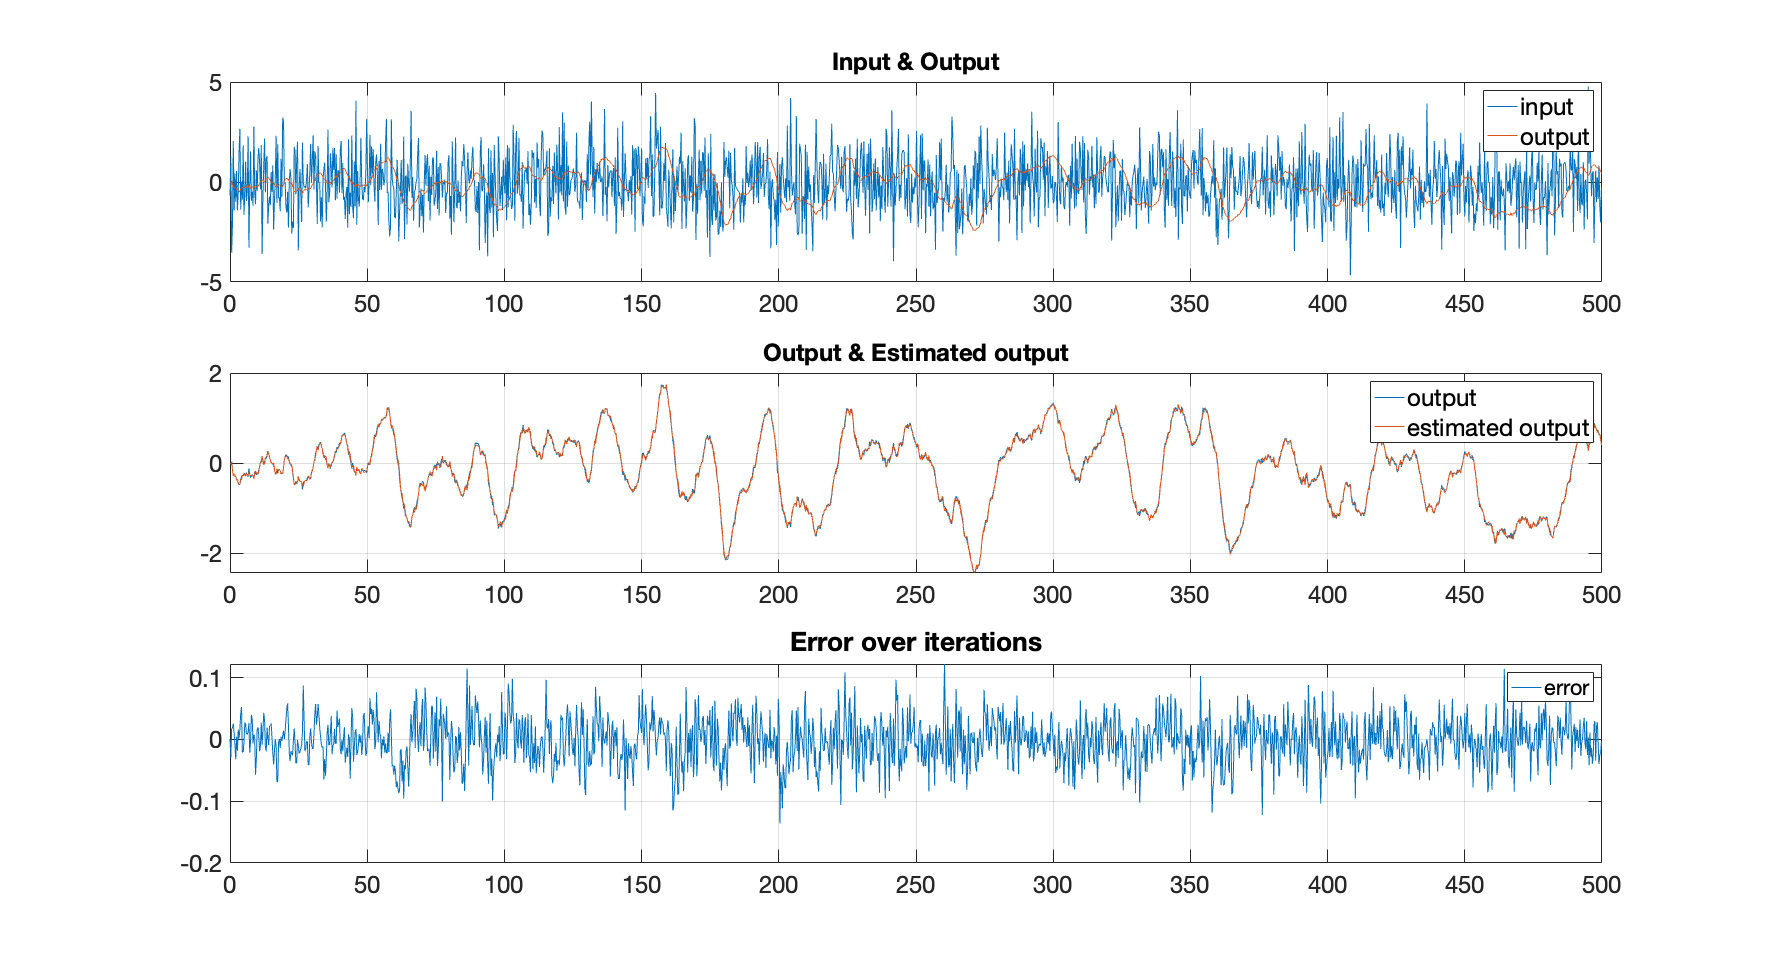
\includegraphics[totalheight=8cm]{images/RLSISPCOutput.png}
\caption{RLS system output with sudden change}
\label{fig:RLSISPCOutput}
\end{figure}
\begin{figure}
\centering
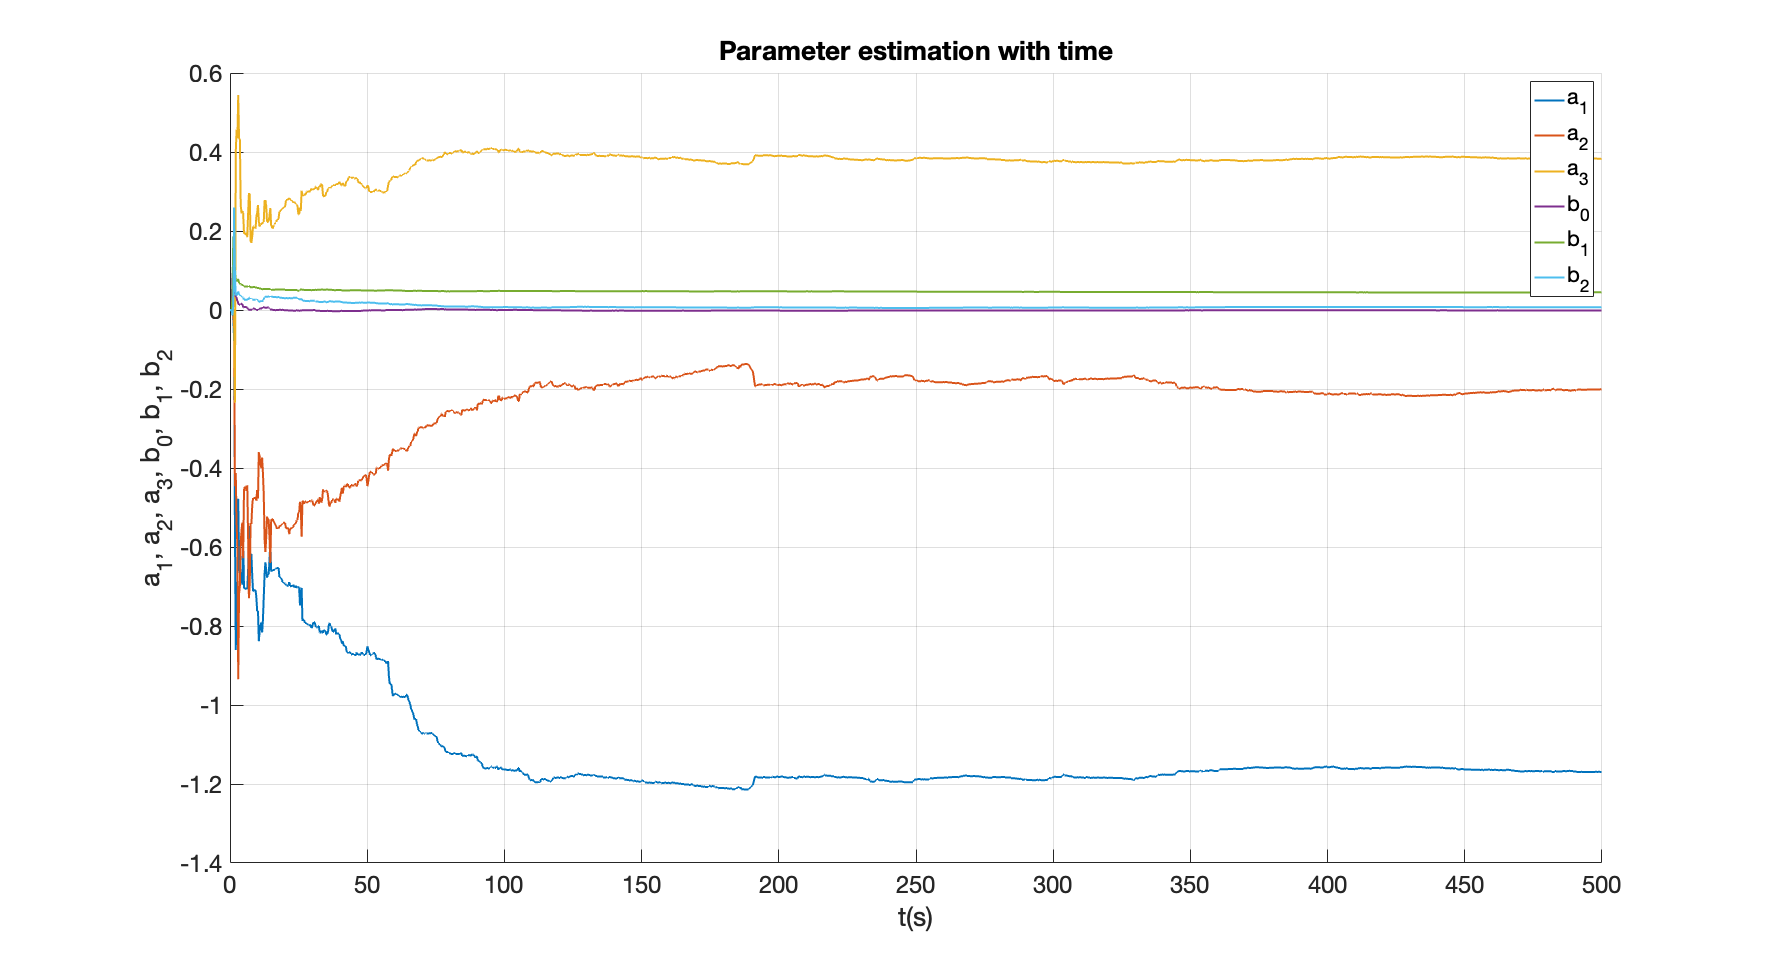
\includegraphics[totalheight=8cm]{images/RLSISPCParams.png}
\caption{RLS system parameters with sudden change}
\label{fig:RLSISPCParams}
\end{figure}
\begin{equation}
G(z) =	\frac{-0.0002047 z^2 + 0.04428 z + 0.008291}{z^3 - 1.155 z^2 - 0.2157 z + 0.3819}
\label{eq:RLSISPCTransferFunction}
\end{equation}

\autoref{fig:RLSISPCFixedOutput} demonstrates the improved system identification, and \autoref{fig:RLSISPCFixedOutputParams} shows the enhanced parameter estimation. The resulting transfer function is presented in \autoref{eq:RLSISPCFixedTransferFunction}.

\begin{figure}
	\centering
	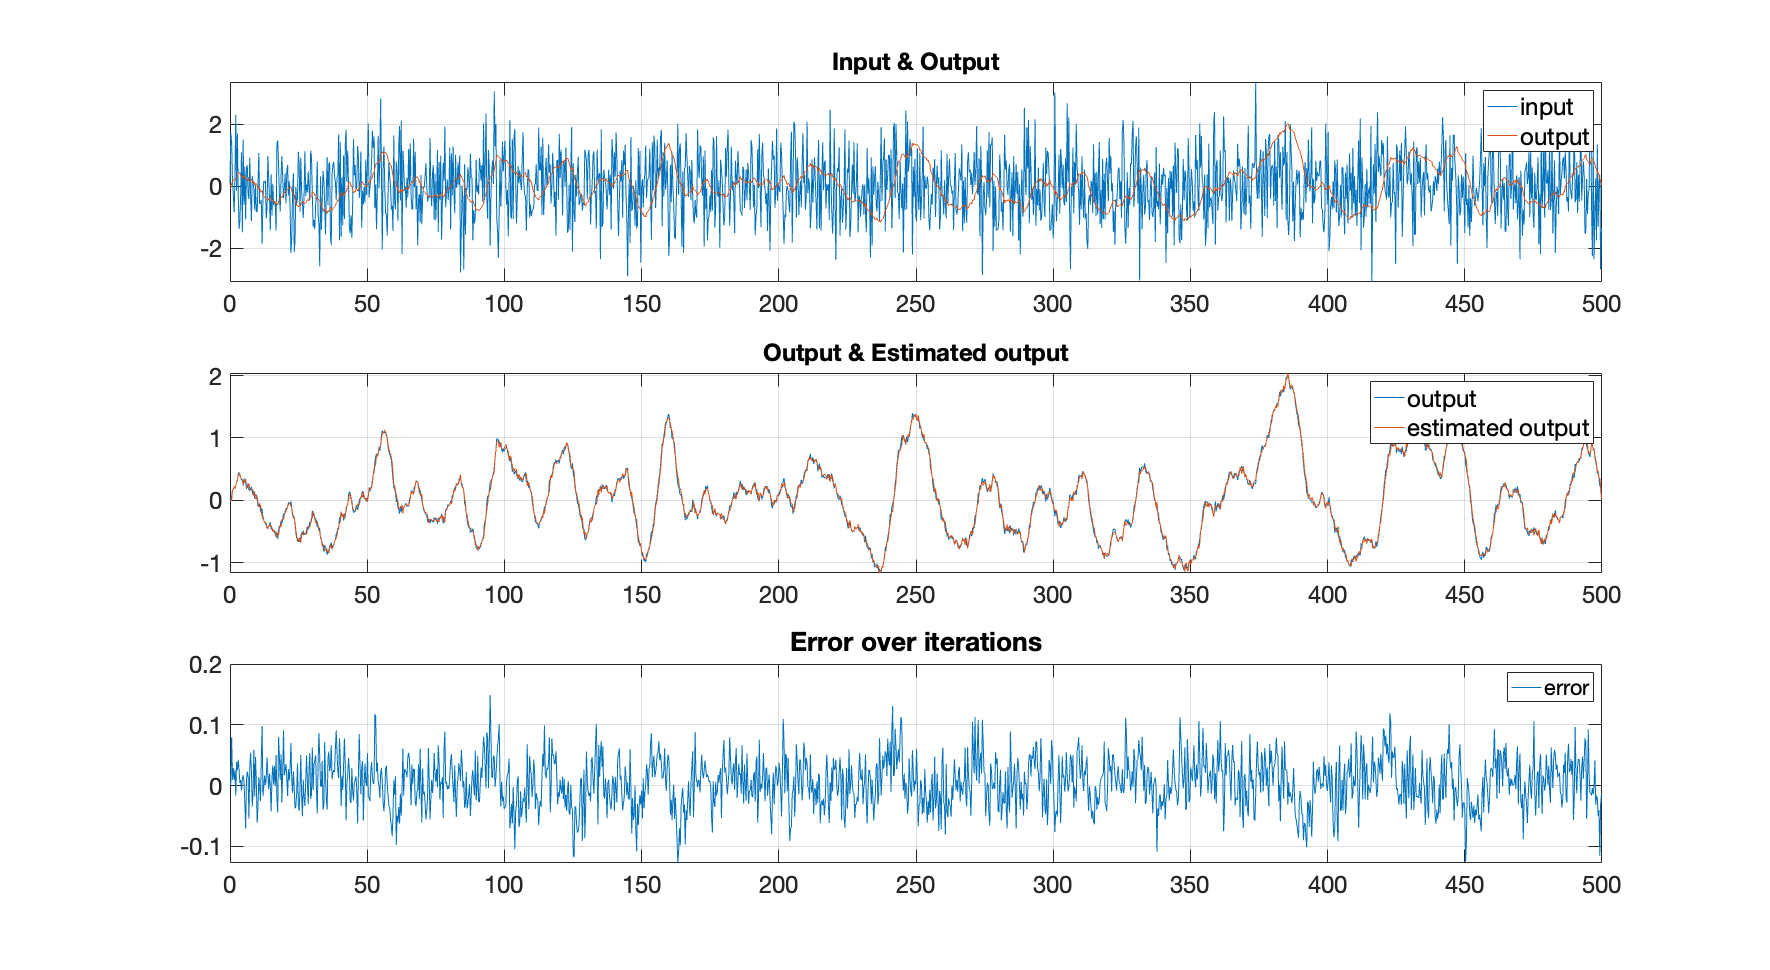
\includegraphics[totalheight=8cm]{images/RLSISPCFixedOutput.png}
	\caption{Improved RLS system output with sudden change}
	\label{fig:RLSISPCFixedOutput}
\end{figure}
\begin{figure}
	\centering
	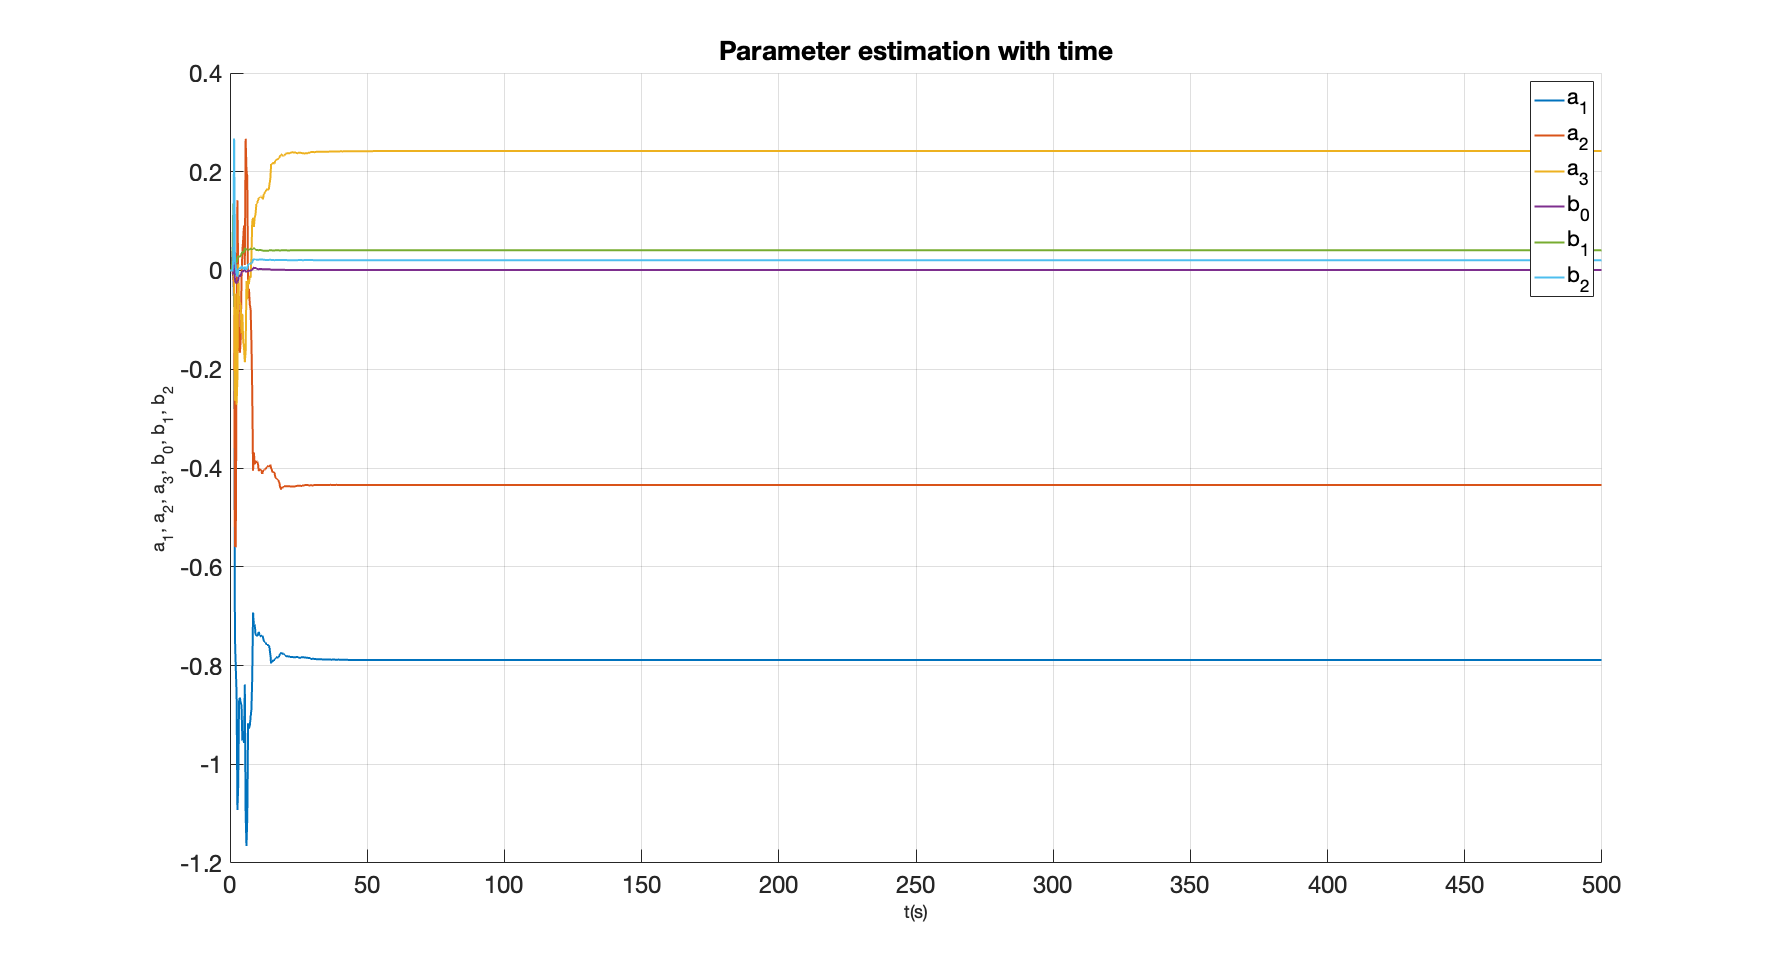
\includegraphics[totalheight=8cm]{images/RLSISPCFixedParams.png}
	\caption{Improved RLS system parameters with sudden change}
	\label{fig:RLSISPCFixedOutputParams}
\end{figure}
\begin{equation}
	G(z) =	\frac{0.00564 z^2 + 0.04625 z + 0.006189}{z^3 - 0.9525 z^2 - 0.3035 z + 0.2608}
	\label{eq:RLSISPCFixedTransferFunction}
\end{equation}

The Simulink model for this section is available at \lstinline|assignment1/part2/2_5/RLS2_5_NS.slx|. The MATLAB code for the system is located at \lstinline|assignment1/part2/2_5/RLS2_5_noise.m|, and the code for the improved system identification is at \lstinline|assignment1/part2/2_5/RLS2_5_fix.m|.
